\documentclass[a4paper, 11pt]{article}

\usepackage{worknote}[title=Android进程相关的]
\title{Android进程相关的\\[2pt]\normalsize 内存、生命周期、任务和活动}

%\usepackage[owner=Donald,user=Knuth,print=false]{pdfcrypt}
%\pdfcrypt{owner "foo" user "bar" none}
\makeindex

\begin{document}
\maketitle
\tableofcontents
\section{Java GC Mechanism}
\subsection{Java是如何管理内存}
为了判断Java中是否有内存泄露,我们首先必须了解Java是如何管理内存的。Java的内存管理就是对象的分配和释放问题。在Java中,程序员需要通过关键字new为每个对象申请内存空间 (基本类型除外),所有的对象都在堆 (Heap)中分配空间。另外,对象的释放是由GC决定和执行的。在Java中,内存的分配是由程序完成的,而内存的释放是有GC完成的,这种收支两条线的方法确实简化了程序员的工作。但同时,它也加重了JVM的工作。这也是Java程序运行速度较慢的原因之一。为了能够正确释放对象,GC必须监控每一个对象的运行状态,包括对象的申请、引用、被引用、赋值等。
\begin{verbatim}
监视对象状态是为了更加准确地、及时地释放对象,而释放对象的根本原则就是该对象不再被引用。
\end{verbatim}

为了更好理解GC的工作原理,我们可以将对象考虑为有向图的顶点,将引用关系考虑为图的有向边,有向边从引用者指向被引对象。另外,每个线程对象可以作为一个图的起始顶点,例如大多程序从main进程开始执行,那么该图就是以main进程顶点开始的一棵根树。在这个有向图中,根顶点可达的对象都是有效对象,GC将不回收这些对象。如果某个对象 (连通子图)与这个根顶点不可达(注意,该图为有向图),那么我们认为这个(这些)对象不再被引用,可以被GC回收。

以下,我们举一个例子说明如何用有向图表示内存管理。对于程序的每一个时刻,我们都有一个有向图表示JVM的内存分配情况。以下右图,就是左边程序运行到第6行的示意图。

\begin{center}
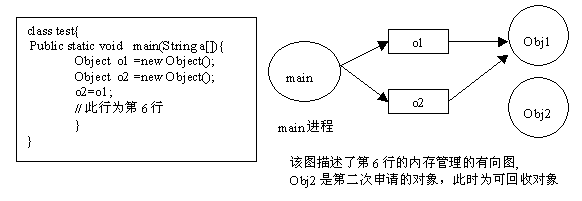
\includegraphics[scale=0.6]{javaobjref.png}
\end{center}

Java使用有向图的方式进行内存管理,可以消除引用循环的问题,例如有三个对象,相互引用,只要它们和根进程不可达的,那么GC也是可以回收它们的。这种方式的优点是管理内存的精度很高,但是效率较低。另外一种常用的内存管理技术是使用计数器,例如COM模型采用计数器方式管理构件,它与有向图相比,精度行低(很难处理循环引用的问题),但执行效率很高。

\subsection{内存泄露}
下面,我们就可以描述什么是内存泄漏。在Java中,内存泄漏就是存在一些被分配的对象
,这些对象有下面两个特点,首先,这些对象是可达的,即在有向图中,存在通路可以与
其相连;其次,这些对象是无用的,即程序以后不会再使用这些对象。如果对象满足这两
个条件,这些对象就可以判定为Java中的内存泄漏,这些对象不会被GC所回收,然而它却
占用内存。

在C++中,内存泄漏的范围更大一些。有些对象被分配了内存空间,然后却不可达,由于
C++中没有GC,这些内存将永远收不回来。在Java中,这些不可达的对象都由GC负责回收
,因此程序员不需要考虑这部分的内存泄露。

通过分析,我们得知,对于C++,程序员需要自己管理边和顶点,而对于Java程序员只需
要管理边就可以了(不需要管理顶点的释放)。通过这种方式,Java提高了编程的效率。
\begin{center}
\includegraphics[scale=0.7]{javamemgc.png}
\end{center}


因此,通过以上分析,我们知道在Java中也有内存泄漏,但范围比C++要小一些。因为Java从语言上保证,任何对象都是可达的,所有的不可达对象都由GC管理。

对于程序员来说,GC基本是透明的,不可见的。虽然,我们只有几个函数可以访问GC,例如运行GC的函数System.gc(),但是根据Java语言规范定义, 该函数不保证JVM的垃圾收集器一定会执行。因为,不同的JVM实现者可能使用不同的算法管理GC。通常,GC的线程的优先级别较低。JVM调用GC的策略也有很多种,有的是内存使用到达一定程度时,GC才开始工作,也有定时执行的,有的是平缓执行GC,有的是中断式执行GC。但通常来说,我们不需要关心这些。除非在一些特定的场合,GC的执行影响应用程序的性能,例如对于基于Web的实时系统,如网络游戏等,用户不希望GC突然中断应用程序执行而进行垃圾回收,那么我们需要调整GC的参数,让GC能够通过平缓的方式释放内存,例如将垃圾回收分解为一系列的小步骤执行,Sun提供的HotSpot JVM就支持这一特性。

下面给出了一个简单的内存泄露的例子。在这个例子中,我们循环申请Object对象,并将所申请的对象放入一个Vector中,如果我们仅仅释放引用本身,那么Vector仍然引用该对象,所以这个对象对GC来说是不可回收的。因此,如果对象加入到Vector后,还必须从Vector中删除,最简单的方法就是将Vector对象设置为null。


\begin{lstlisting}
Vector v=new Vector(10);
for (int i=1;i<100; i++)
{
	Object o=new Object();
	v.add(o);
	o=null;	
} 
\end{lstlisting}


\subsection{Android Memory Leak}
\begin{lstlisting}[language=java,]
public class Blackboard extends Activity {
    private final static String TAG = "MemoryLeakTest";

    Bitmap mBitmap;
    byte mass[];
    private static Drawable mBackground;
    static List<byte[]> mRawData = new ArrayList<byte[]>();

    public void onCreate(Bundle savedInstanceState) {
        super.onCreate(savedInstanceState);        

        MemoryProbe.showMemory("onCreate");

        TextView label = new TextView(this);
        label.setText("Leaks are bad");

        if (mBackground == null) {
            mBackground = getResources().getDrawable(R.drawable.greatwall);
        } 
        mBitmap = BitmapFactory.decodeResource(getResources(), R.drawable.greatwall); 
        label.setBackgroundDrawable(mBackground); 
        setContentView(label); 

        //staticCollectionLeak();
        //fileLeakTest();
        //cursorLeakTest();
        //registerLeakTest();
        contentObserverLeakTest();
    }

    /*
     * 测试结果: 造成 dalvik 的内存泄漏。 hprof 可以定位。
     */
    private void staticCollectionLeak() {
        mass = new byte[8 * 1024 * 1024];
        mRawData.add(mass);  //内存泄漏.  
    }

    /*
     * 测试结果:IO 未 close 不会造成内存泄漏 
     */
    private void fileLeakTest( ) {
        try{
            FileOutputStream fos;
            int i = 0;
            String contents = "Write some test to file\n";
            fos = openFileOutput("fileLeakTest.txt", MODE_PRIVATE);
            while (i++ < 1000) {
                fos.write(contents.getBytes());
            }
        } catch (Exception e) {
            Log.e(TAG, "oops, catch Exception " + e);
        } finally {
            //fos.close();
        }
    }

    /*
     * 测试结果: IntentFilter 未 unregisterReceiver 会造成native内存泄漏。 但当进程
     *                  重启时会报错:
     * ActivityThread    Activity com.sibrary.classroom.Blackboard has leaked IntentReceiver com.sibrary.classroom.Blackboard$1@40525d08 that was originally registe
     red here. Are you missing a call to unregisterReceiver()?
     ActivityThread    android.app.IntentReceiverLeaked: Activity com.sibrary.classroom.Blackboard has leaked IntentReceiver com.sibrary.classroom.Blackboard$1@40
     525d08 that was originally registered here. Are you missing a call to unregisterReceiver()?
     ActivityThread  at android.app.LoadedApk$ReceiverDispatcher.<init>(LoadedApk.java:756)
     ActivityThread  at android.app.LoadedApk.getReceiverDispatcher(LoadedApk.java:551)
     ActivityThread  at android.app.ContextImpl.registerReceiverInternal(ContextImpl.java:803)

*/
    private void registerLeakTest() {
        IntentFilter filter = new IntentFilter();
        filter.addAction(Intent.ACTION_DATE_CHANGED);
        filter.addAction(Intent.ACTION_BATTERY_CHANGED);
        registerReceiver(mIntentReceiver, filter);
    }

    /*
     * 测试结果: 未unregisterContentObserver 时会造成 native 内存泄漏。
     */
    private void contentObserverLeakTest() {
        getContentResolver().registerContentObserver(Settings.System.CONTENT_URI, true, mDateFomat);
    }

    /*
     * 测试结果: Cursor 未 close 时不会造成内存泄漏。 但是会有如下警告,有时
     * 要多测几次:
     *  1123       StrictMode  E  Finalizing a Cursor that has not been deactivated or closed. database = /data/data/com.android.soundrecorder/databases/simple, table = soun
                           drecorder, query = SELECT * FROM soundrecorder ORDER BY _id
 1123       StrictMode  E  android.database.sqlite.DatabaseObjectNotClosedException: Application did not close the cursor or database object that was opened here
 1123       StrictMode  E  	at android.database.sqlite.SQLiteCursor.<init>(SQLiteCursor.java:214)
 1123       StrictMode  E  	at android.database.sqlite.SQLiteDirectCursorDriver.query(SQLiteDirectCursorDriver.java:53)

     */

    private void cursorLeakTest() {
        String[] projection = new String[] {Media._ID, Media.TITLE};
        Cursor cursorImage = managedQuery(Media.EXTERNAL_CONTENT_URI, projection, null, null, 
                Media.DATE_TAKEN + " ASC");
    }

    @Override
    protected void onDestroy() {	
        super.onDestroy();
        MemoryProbe.showMemory("onDestroy");
    }

    private final ContentObserver mDateFomat = 
        new ContentObserver(new Handler()) {
            public void onChange(boolean selfChange) {
            }
    };

    private final BroadcastReceiver mIntentReceiver = new BroadcastReceiver() {
        public void onReceive(Context context, Intent intent) {
            final String action = intent.getAction();
            if (Intent.ACTION_DATE_CHANGED.equals(action)) {
            } else if (Intent.ACTION_BATTERY_CHANGED.equals(action)) {
            }
        }
    };
}
\end{lstlisting}

其中,最难发觉的是 registerContentObserver, 这个是native 泄漏, hprof 是没法
察觉的,而 2.3.5 的logcat 上也看不到。

\section{进程管理}
\subsection{Android Process}
Android采取了一种有别于Linux的进程管理策略,有别于Linux的在进程活动停止后就结束该进程,Android把这些进程都保留在内存中,直到系统需要更多内存为止。这些保留在内存中的进程通常情况下不会影响整体系统的运行速度,并且当用户再次激活这些进程时,提升了进程的启动速度。

那Android什么时候结束进程?结束哪个进程呢?之前普遍的认识是Android是依据一个名为LRU(last recently used 最近使用过的程序)列表,将程序进行排序,并结束最早的进程。XDA的楼主又进一步对这个管理机制进行研究,有了如下发现:

系统会对进程的重要性进行评估,并将重要性以“oom_adj”这个数值表示出来,赋予各个进程;(系统会根据“oom_adj”来判断需要结束哪些进程,一般来说,“oom_adj”的值越大,该进程被系统选中终止的可能就越高)
前台程序的“oom_adj”值为0,这意味着它不会被系统终止,一旦它不可访问后,会获得个更高的“oom_adj”,作者推测“oom_adj”的值是根据软件在LRU列表中的位置所决定的;
Android不同于Linux,有一套自己独特的进程管理模块,这个模块有更强的可定制性,可根据“oom_adj”值的范围来决定进程管理策略,比如可以设定“当内存小于X时,结束“oom_adj”大于Y的进程”。这给了进程管理脚本的编写以更多的选择。

Android将进程分为六大类:
\begin{enumerate}
    \item 前台进程(foreground):目前正在屏幕上显示的进程和一些系统进程。举例来说,Dialer Storage,Google Search等系统进程就是前台进程;再举例来说,当你运行一个程序,如浏览器,当浏览器界面在前台显示时,浏览器属于前台进程(foreground),但一旦你按home回到主界面,浏览器就变成了后台程序(background)。我们最不希望终止的进程就是前台进程。
    \item 可见进程(visible):可见进程是一些不在前台,但用户依然可见的进程,举个例来说:widget、输入法等,都属于visible。这部分进程虽然不在前台,但与我们的使用也密切相关,我们也不希望它们被终止(你肯定不希望时钟、天气,新闻等widget被终止,那它们将无法同步,你也不希望输入法被终止,否则你每次输入时都需要重新启动输入法)
    \item 次要服务(secondary server):目前正在运行的一些服务(主要服务,如拨号等,是不可能被进程管理终止的,故这里只谈次要服务),举例来说:谷歌企业套件,Gmail内部存储,联系人内部存储等。这部分服务虽然属于次要服务,但跟一些系统功能依然息息相关,我们时常需要用到它们,所以也不希望他们被终止
    \item 后台进程(hidden):虽然作者用了hidden这个词,但实际即是后台进程(background),就是我们通常意义上理解的启动后被切换到后台的进程,如浏览器,阅读器等。当程序显示在屏幕上时,它所运行的进程即为前台进程(foreground),一旦我们按home返回主界面(注意是按home,不是按back),程序就驻留在后台,成为后台进程(background)。后台进程的管理策略有多种:有较为积极的方式,一旦程序到达后台立即终止,这种方式会提高程序的运行速度,但无法加速程序的再次启动;也有较消极的方式,尽可能多的保留后台程序,虽然可能会影响到单个程序的运行速度,但在再次启动已启动的程序时,速度会有所提升。这里就需要用户根据自己的使用习惯找到一个平衡点
    \item 内容供应节点(content provider):没有程序实体,仅提供内容给别的程序去用的,比如日历供应节点,邮件供应节点等。在终止进程时,这类程序应该有较高的优先权
    \item 空进程(empty):没有任何东西在内运行的进程,有些程序,比如BTE,在程序退出后,依然会在进程中驻留一个空进程,这个进程里没有任何数据在运行,作用往往是提高该程序下次的启动速度或者记录程序的一些历史信息。这部分进程无疑是应该最先终止的。
\end{enumerate}

特征:
1.如果一个进程里面同时包含service和可视的activity,那么这个进程应该归于可视进程,而不是service进程。
2.另外,如果其他进程依赖于它的话,一个进程的等级可以提高。例如,一个A进程里的service被绑定到B进程里的组件上,进程A将总被认为至少和B进程一样重要。
3.系统中的phone服务被划分到前台进程而不是次要服务进程.

如果一个进程(或者说apk)只有 service 和 receiver,而没有 activity, 而这个
service 只被receiver 启动,别的进程被未关联,那么,在运行 40分钟后,进程被重启
,这是 2.3.5 中观察到的现象。

Android主要应用在嵌入式设备当中,而嵌入式设备由于一些众所周知的条件限制,通常都不会有很高的配置,特别是内存是比较有限的。如果我们编写 的代码当中有太多的对内存使用不当的地方,难免会使得我们的设备运行缓慢,甚至是死机。为了能够使得Android应用程序安全且快速的运 行,Android的每个应用程序都会使用一个专有的Dalvik虚拟机实例来运行,它是由Zygote服务进程孵化出来的,也就是说每个应用程序都是在 属于自己的进程中运行的。一方面,如果程序在运行过程中出现了内存泄漏的问题,仅仅会使得自己的进程被kill掉,而不会影响其他进程(如果是 system_process等系统进程出问题的话,则会引起系统重启)。另一方面Android为不同类型的进程分配了不同的内存使用上限,如果应用进 程使用的内存超过了这个上限,则会被系统视为内存泄漏,从而被kill掉。Android为应用进程分配的内存上限如下所示:
位置: /ANDROID_SOURCE/system/core/rootdir/init.rc 部分脚本
\begin{lstlisting}[language=,]
# Define the oom_adj values for the classes of processes that can be
# killed by the kernel. These are used in ActivityManagerService.
  setprop ro.FOREGROUND_APP_ADJ 0
  setprop ro.VISIBLE_APP_ADJ 1
  setprop ro.SECONDARY_SERVER_ADJ 2
  setprop ro.BACKUP_APP_ADJ 2
  setprop ro.HOME_APP_ADJ 4
  setprop ro.HIDDEN_APP_MIN_ADJ 7
  setprop ro.CONTENT_PROVIDER_ADJ 14
  setprop ro.EMPTY_APP_ADJ 15
# Define the memory thresholds at which the above process classes will
# be killed. These numbers are in pages (4k).
  setprop ro.FOREGROUND_APP_MEM 1536
  setprop ro.VISIBLE_APP_MEM 2048
  setprop ro.SECONDARY_SERVER_MEM 4096
  setprop ro.BACKUP_APP_MEM 4096
  setprop ro.HOME_APP_MEM 4096
  setprop ro.HIDDEN_APP_MEM 5120
  setprop ro.CONTENT_PROVIDER_MEM 5632
  setprop ro.EMPTY_APP_MEM 6144
# Write value must be consistent with the above properties.
# Note that the driver only supports 6 slots, so we have HOME_APP at the
# same memory level as services.
  write /sys/module/lowmemorykiller/parameters/adj 0,1,2,7,14,15
  write /proc/sys/vm/overcommit_memory 1
  write /proc/sys/vm/min_free_order_shift 4
  write /sys/module/lowmemorykiller/parameters/minfree 1536,2048,4096,5120,5632,6144
  # Set init its forked children's oom_adj.
  write /proc/1/oom_adj -16
\end{lstlisting}
  正因为我们的应用程序能够使用的内存有限,所以在编写代码的时候需要特别注意内存使用问题。
进程的oom_adj值也就代表了它的优先级。oom_adj值越高代表该进程优先级越低。
/init.rc中,将PID为1的进程(init进程)的oom_adj设置为SYSTEM_ADJ(-16)。

查看本机设置:
cat /sys/module/lowmemorykiller/parameters/adj
0,1,2,7,14,15
 
回收时机:
文件/init.rc中:
\begin{lstlisting}[language=,]
   setprop ro.FOREGROUND_APP_MEM       1536     // 6M
   setprop ro.VISIBLE_APP_MEM          2048     // 8M
   setprop ro.SECONDARY_SERVER_MEM     4096     // 16M
   setprop ro.HIDDEN_APP_MEM           5120     // 20M
   setprop ro.CONTENT_PROVIDER_MEM     5632     // 22.4M
   setprop ro.EMPTY_APP_MEM            6144     // 24M
\end{lstlisting}
这些数字也就是对应的内存阈值,一旦低于该值,Android便开始按顺序关闭相应等级的进程。
注意这些数字的单位是page: 1 page = 4 kB。所以上面的六个数字对应的就是(MB): 6,8,16,20,22,24。
 
查看现在的内存阈值设置:

\lstinline{cat /sys/module/lowmemorykiller/parameters/minfree}

要想重新设置该值(对应不同的需求):

\lstinline{echo "1536,2048,4096,5120,15360,23040">/sys/module/lowmemorykiller/parameters/minfree}

这样当可用内存低于90MB的时候便开始杀死"空进程",而当可用内存低于60MB的时候才开始杀死"内容供应节点"类进程。
 
具体的回收实现在ActivityManagerService.java中的函数trimApplications():
\begin{lstlisting}[language=,]
   1.首先移除 package 已被卸载的无用进程;
   2.基于进程当前状态,更新 oom_adj 值,然后进行以下操作:
         1) 移除没有 activity 在运行的进程;
         2) 如果AP已经保存了所有的 activity 状态,结束这个AP。
   3. 最后,如果目前还是有很多 activities 在运行,那么移除那些 activity
   状态已经保存好的 activity 。
\end{lstlisting}
 

更新oom_adj的值:
在ActivityManagerService.java文件的ComputeOomAdjLocked() 中计算出进程的oom_adj,例如:
\begin{lstlisting}
     if (app == TOP_APP) {
            // The last app on the list is the foreground app.
            adj = FOREGROUND_APP_ADJ;
            app.adjType = "top-activity";
        }
\end{lstlisting}
 
Android kernel中的low memory killer
Android的Low Memory Killer根据需要(当系统内存短缺时)杀死进程释放其内存,源代码在kernel/drivers/misc/lowmemorykiller.c中。简单说,就是寻找一个最合适的进程杀死,从而释放它占用的内存。
最合适的进程是:
   •  oom_adj越大
   •  占用物理内存越多
 
一旦一个进程被选中,内核会发送SIGKILL信号将之杀死:
\begin{lstlisting}
   for_each_process(p) {
        ……
        if(selected == NULL ||   p->oomkilladj > selected->oomkilladj ||
              (p->oomkilladj == selected->oomkilladj && tasksize > selected_tasksize))
        {
             selected = p;
        }
   }
   if(selected != NULL) {
        force_sig(SIGKILL, selected);
   }
\end{lstlisting}
 
查看LRU列表:adb shell dumpsys activity
当activitydemo在前台时: 
包含Service的进程的优先级比较高,在computeOomAdjLocked中将其分为了两小类:
\begin{lstlisting}
      static final int MAX_SERVICE_INACTIVITY = 30*60*1000;                 
      if (now < (s.lastActivity+MAX_SERVICE_INACTIVITY)) {
               if (adj > SECONDARY_SERVER_ADJ) {
                            adj = SECONDARY_SERVER_ADJ;
                            app.adjType = "started-services";
                            app.hidden = false;
               }
      }
      if (adj > SECONDARY_SERVER_ADJ) {
                        app.adjType = "started-bg-services";
      }
\end{lstlisting}
 

完全让进程不被kill是不可能的,我们可以通过一些操作,使进程被kill的几率变小:
  1) 提高进程的优先级:
        * 后台操作采用Service形式,因为一个运行着service的进程比一个运行着后台activity的等级高;
        * 按back键使得进程中的activity在后台运行而不是destory,需重载back按键(没有任何activity在运行的进程优先被杀).
        * 依赖于其他优先级高的进程;

  2) 强制修改进程属性:
        * 在进程中设置:setPersistent(true);
        * 在Manifest文件中设置(如上)。

\subsection{本地内存和Java内存}
\begin{lstlisting}
09-28 17:16:37.543: DEBUG/dalvikvm(21466): GC_EXTERNAL_ALLOC freed 390 objects / 45656 bytes in 50ms
09-28 17:16:40.513: DEBUG/dalvikvm(3267): GC_EXPLICIT freed 4501 objects / 251624 bytes in 67ms
\end{lstlisting}

很多做开发的朋友不明白上面这句是什么意思,给大家解释一下!
前面Free的内存是VM中java使用的内存,external是指VM中通过JNI中Native的类中的malloc分配出的内存,例如Bitmap和一些Cursor都是这么分配的。

在Davilk中,给一个程序分配的内存根据机型厂商的不同,而不同,现在的大部分的是32M了,而在VM内部会把这些内存分成java使用的内存和 Native使用的内存,它们之间是不能共享的,就是说当你的Native内存用完了,现在Java又有空闲的内存,这时Native会重新像VM申请,而不是直接使用java的。

例如上边的例子
free 3411K/6663K和external 24870K/26260K

如果这时需要创建一个2M的Bitmap,Native现有内存26260-24870=1390K < 2048k,因此他就会向Vm申请内存,虽然java空闲
的内存是6663-3411=3252>2048,但这部分内存Native是不能使用。

但是你现在去申请2M的Native内存,VM会告诉你无法分配的,因为现在已使用的内存已经接近峰值了32M(26260+6663=32923 ),所以现在就会成force close 报OOM。

所以现在我们要检查我们的native内存的使用情况来避免OOM。

adb shell dumpsys meminfo 

\subsection{避免进程被杀死}
对于放在/system/app下的应用,需要设置persistent属性,如应用程序'Phone'的AndroidManifest.xml文件:
\begin{lstlisting}
    <application android:name="PhoneApp"
                 android:persistent="true"
                 android:label="@string/dialerIconLabel"
                 android:icon="@drawable/ic_launcher_phone">
         ...
    </application>
\end{lstlisting}
设置后app提升为系统核心级别,任何情况下不会被kill掉, settings->applications里面也会屏蔽掉stop操作。

这样设置前的log:  
\begin{lstlisting}[language=,]
Proc #19: adj=svc  /B 4067b028 255:com.xxx.xxx/10001 (started-services)
# cat /proc/255/oom_adj
    4
\end{lstlisting}
设置后的log:
\begin{lstlisting}[language=,]
PERS #19: adj=core /F 406291f0 155:com.xxx.xxx/10001 (fixed)
    # cat /proc/155/oom_adj
     -12                # 这是CORE_SERVER_ADJ
\end{lstlisting}
注:init进程的oom_adj为-16(即SYSTEM_ADJ):
cat  /proc/1/oom_adj

在文件frameworks/base/services/java/com/android/server/am/ActivityManagerService.java中有以下的代码:
\begin{lstlisting}
    final ProcessRecord addAppLocked(ApplicationInfo info) {
        ProcessRecord app = getProcessRecordLocked(info.processName, info.uid);

        if (app == null) {
            app = newProcessRecordLocked(null, info, null);
            mProcessNames.put(info.processName, info.uid, app);
            updateLruProcessLocked(app, true, true);
        }    

        if ((info.flags&(ApplicationInfo.FLAG_SYSTEM|ApplicationInfo.FLAG_PERSISTENT))
                == (ApplicationInfo.FLAG_SYSTEM|ApplicationInfo.FLAG_PERSISTENT)) {
            app.persistent = true;
            app.maxAdj = CORE_SERVER_ADJ;             // 这个常数值为 -12 。
        }    
        if (app.thread == null && mPersistentStartingProcesses.indexOf(app) < 0) {
            mPersistentStartingProcesses.add(app);
            startProcessLocked(app, "added application", app.processName);
        }    

        return app;
    }
\end{lstlisting}

可见要想成为core service (即app.maxAdj = CORE_SERVER_ADJ(-12)),
应用程序需要FLAG_SYSTEM和FLAG_PERSISTENT两个标志,
FLAG_SYSTEM指的是应用位于/system/app下,FLAG_PERSISTENT就是指persistent属性。

而对于frameworks/base/services/java/com/android/server/SystemServer.java,则调用
       ActivityManagerService.setSystemProcess();
把自己的 app.maxAdj 设置成SYSTEM_ADJ,即-16。

\subsection{进程、任务和活动}
顺便搞清楚三者关系。
关于Android中的组件和应用,当然是基于进程、线程。在Android中,组件的动态运行,有一个最与众不同的概念,就是Task,翻译成任务,应该还是比较顺理成章的。
Task的介入,最主要的作用,是将组件之间的连接,从进程概念的细节中剥离出来,可以以一种不同模型的东西进行配置,在很多时候,能够简化上层开发人员的理解难度,帮助大家更好的进行开发和配置。


以往基于应用(application)的程序开发中,程序具有明确的边界,一个程序就是一个应用,一个应用为了实现功能可以采用开辟新线程甚至新进程来辅助,但是应用与应用之间不能复用资源和功能。而Android引入了基于组件开发的软件架构,虽然我们开发android程序,仍然使用一个apk工程一个Application的开发形式,但是对于Aplication的开发就用到了Activity、service等四大组件,其中的每一个组件,都是可以被跨应用复用的哦,这个就是android的神奇之处。
另外值得一提的是,虽然组件可以跨应用被调用,但是一个组件所在的进程必须是在组件所在的Aplication进程中。由于android强化了组件概念,弱化了Aplication的概念,所以在android程序开发中,A应用的A组件想要使用拍照或录像的功能就可以不用去针对Camera类进行开发,直接调用系统自带的摄像头应用(称其B应用)中的组件(称其B组件)就可以了,但是这就引发了一个新问题,A组件跑在A应用中,B组件跑在B应用中,自然都不在同一个进程中,那么从B组件中返回的时候,如何实现正确返回到A组件呢?Task就是来负责实现这个功能的,它是从用户角度来理解应用而建立的一个抽象概念。因为用户所能看到的组件就是Activity,所以Task可以理解为实现一个功能而负责管理所有用到的Activity实例的栈。

找一个Task任务最直观的体现吧。先重启手机,长按home键,发现弹出的最近任务中一个任务也没有,然后开启A应用,长按home键,会发现有一个A应用的任务,查看手机进程,应该还没有B进程的;在A应用的A组件中调B应用的B组件,此时看手机的进程,除了A进程外,还有个B的进程,但是长按home键,能看到的还是只有一个A应用的任务。其实这个时候,B应用已经跑起来了,但是对用户来说,他其实没有开启过B应用,所以Task任务自始至终都是从用户的角度出发而设计的概念,保证用户的调用逻辑。


默认情况下,同一个应用程序中的所有组件运行在同一个进程中,而且绝大多数的应用程序也都是这样的。但是,如果我们想要控制让某个特定的组件属于某个进程,我们可以在manifest文件中进行配置。 
在每种组件元素(activity、service、receiver、provider)的manifest条目中,都支持一个 “android:process”的属性,通过这个属性,我们可以指定某个组件运行的进程。我们可以通过设置这个属性,让每个组件运行在它自己的进程中,也可以只让某些组件共享一个进程。我们要可以通过设置“android:process”属性,让不同应用程序中的组件运行在相同的进程中,这些应用程序共享相同的Linux用户ID,拥有相同的证书。 
<application>元素也有一个“android:process”属性,可以设置一个应用于全部组件的默认值。 
    当可用内存数量低,而一些与用户即时交互的进程又需要内存时,Android随时可能会终止某个进程。运行在被终止的进程中的组件会因此被销毁,但是,当再次需要这些组件工作时,就会再启动一个进程。 
    在决定要终止哪个进程时,Android系统会权衡它们对于用户的重要性。例如,相较于运行可见activities的进程,终止一个运行不可见activities的进程会更加合理。是否终止一个进程,依赖于运行在这个进程中的组件的状态。 
如果不能将两个activity放入同一个application中的话,可以通过在各自的manifest中设置以下属性,让这两个activity强制运行在同一个进程中,从而可以充分利用进程内共享的资源,减少内存占用:
\begin{verbatim}
(1)设置相同的User Id:  
<manifest android:sharedUserId="aaa.bbb"  
(2)被调用的activity设置以下属性:  
        1. <activity android:multiprocess="true"  
        2.  <activity android:process="com.cienet.test"  

\end{verbatim}

一个 Activity 可以启动另一个,即便是定义在不同应用程序中的 Activity 。例如,假设你想让用户显示一些地方的街景。而这里已经有一个 Activity 可以做到这一点,因此,你的 Activity 所需要做的只是在 Intent 对象中添加必要的信息,并传递给 startActivity() 。地图浏览将会显示你的地图。当用户按下 BACK 键,你的 Activity 会再次出现在屏幕上。
 
对于用户来说,看起来好像是地图浏览与你的 Activity 一样,属于相同的应用程序,即便是它定义在其它的应用程序里,并 运行在那个应用程序的进程里。 Android 通过将这两个 Activity 保存在同一个 Task 里来体现这一用户体验。简单来说,一个 Task 就是用户体验上的一个“应用”。它将相关的 Activity 组合在一起,以 stack 的方式管理。 stack 中根 Activity 启动 Task ——典型的,它就是用户在应用程序启动栏中选择的 Activity 。位于 stack 顶端的 Activity 是当前正在运行的——能够聚焦用户的动作。当一个 Activity 启动另一个,新的 Activity 进入 stack ;它成为正在运行的 Activity 。之前的 Activity 仍保留在 stack 中。当用户按下 BACK 键,当前的 Activity 从 stack 中退出,之前的那个成为正在运行的 Activity 。
 
stack 包含对象,因此,如果一个 Task 中有多个同一个 Activity 的实例时——多个地图浏览,例如—— stack 为每个实例拥有一个独立的入口。位于 stack 中的 Activity 不会重新调整,只是进入和退出。
 
一个 Task 就是一组 Activity ,不是一个类或者在 manifest 中定义的一个元素。因此,没有办法为 Task 设置独立于它的 Activity 的属性值。 Task 的值作为整体在根 Activity 中设置。例如,下一个章节会讨论 Task 的“ affinity ”;那个值就是从 Task 中的根 Activity 中读取的。
 
Task 中的所有 Activity 作为一个单元一起移动。整个 Task (整个 Activity stack )可以进入前台或者退到后台。例如,假设当前 Task 中的 stack 中有 4 个 Activity —— 3 个位于当前 Activity 下方。用户按下 HOME 键,进入到应用程序启动栏,然后选择一个新的应用程序(实际上, 一个新的 Task )。当前 Task 退到后台,并且新 Task 中的根 Activity 会显示出来。然后,经过一段时间后,用户回到 Home 画面,然后再次选择前一个应用程序(前一个 Task )。那个拥有 4 个 Activity 的 Task 会进入前台。当用户按下 BACK 键,屏幕不会显示用户刚刚离开的 Activity (前一个 Task 的根 Activity )。而是,这个 stack 中的顶端 Activity 移除,相同 Task 中的前一个 Activity 会显示出来。
 
刚才描述的行为是 Activity 和 Task 的默认行为。但有方法来完全改变它。 Task 之间的关联,和一个 Task 中的一个 Activity 行为,受启动 Activity 的 Intent 对象中设置的 Flag 和 manifest 文件中 Activity 的 <activity> 元素的特性值交互控制。调用者和响应者都有权决定如何发生。

activity和task之间的联系,以及task中的 activity的行为可以通过intent中的标记 以 及在manifest中的<activity>元素 的属性 控制。其中,主要的Intent标记有:
\begin{verbatim}
FLAG_ACTIVITY_NEW_TASK
FLAG_ACTIVITY_CLEAR_TOP
FLAG_ACTIVITY_RESET_TASK_IF_NEEDED
FLAG_ACTIVITY_SINGLE_TOP
\end{verbatim}

主要的<activity>属性有:
\begin{verbatim}
taskAffinity
launchMode
allowTaskReparenting
clearTaskOnLaunch
alwaysRetainTaskState
finishOnTaskLaunch
\end{verbatim}
默认情况下,一个应用程序中的所有activity都有一个affinity–这让它们属性同一个task。然而,每个activity可以通 过<activity>中的taskAffinity属性设置单独的affinity。不同应用程序中的activity可以共享同一个 affinity,同一个应用程序中的不同activity也可以设置成不同的affinity。

affinity属性在2种情况下起作用:

    1. 启动 activity的Intent对象包含FLAG_ACTIVITY_NEW_TASK标记

    2.  activity的 allowTaskReparenting被设置成true。 

当传递给startActivity()的Intent对象包含 FLAG_ACTIVITY_NEW_TASK标记时,系统会为需要启动的activity寻找与当前activity不同的task。如果要启动的 activity的affinity属性与当前所有的task的affinity属性都不相同,系统会新建一个带那个affinity属性的task,并 将要启动的activity压到新建的task栈中;否则将activity压入那个affinity属性相同的栈中。

如果一个activity的allowTaskReparenting属性为true, 那么它可以从一个task(TASK1)移到另外一个有相同affinity的task(TASK2)中(TASK2带到前台时)。
如果一个.apk文件从用户角度来看包含了多个“应用程序”,你可能需要对那些 activity赋不同的affinity值。

activity的launchMode属性可以有四种值:
\begin{itemize}
    \item standard (默认)
    \item singleTop
    \item singleTask
    \item singleInstance
\end{itemize}

以下假设位于task1中的activity1启动activity2:

\littlehb
\begin{multicols}{2}
\begin{itemize}
    \item standard

如果activity2不包含FLAG_ACTIVITY_NEW_TASK标记,则放入task1,否则按前面讲述的规则为activity2选择task

可被多次实例化,同一个task的不同的实例可位于不同的task中,每个task也可包含多个实例

当接收到新的intent时,总是会生成新的activity对象。

\item singleTop

同standard, 如果activity2不包含FLAG_ACTIVITY_NEW_TASK标记,则放入task1,否则按前面讲述的规则为activity2选择task

同standard,可被多次实例化,同一个task的不同的实例可位于不同的task中,每个task也可包含多个实例

但是,已存在的activity对象,如果位于目标task的栈顶,则该activity被重用, 如果它不位于栈顶,则会实例化新的activity对象
\end{itemize}
\end{multicols}
\littlehb
\begin{multicols}{2}
\begin{itemize}

\item singleTask

将activity2放到task1栈底

不能有多个实例。由于该模式下activity总是位于栈顶,所以actvity在同一个设 备里至多只有一个实例

singleTask模式的activity总是位于栈底位置。目标activity 实例已存在时,如果该实例刚好位于task栈顶,则接收intent,否则到来的intent将会被丢弃,但该可以响应该intent的那个 activity所在的task将会被移到前台。

\item singleInstance

将activity2放到task1栈底

不能有多个实例。由于该模式下activity总是位于栈顶,所以actvity在同一个设 备里至多只有一个实例

不允许与其它activity共存于一个task。如果activity1的运行在该模式 下,则activity2一定与activity1位于不同的task
\end{itemize}
\end{multicols}
\littlehb

对于新到的intent,如果是由新创建的activity对象来接收,则用户可以通过返回键回到之前的activity;如果是由已存在的 activity来接收,则用户无法通过返回键返回到接收intent之前的状态。

清空栈

当用户长时间离开task(当前task被转移到后台)时,系统会清除task中栈底activity外的所有activity。这样,当用户返回 到task时,只留下那个task最初始的activity了。
这是默认的情况,<activity>中有些属性可以改变这种行为。
\begin{itemize}
    \item alwaysRetainTaskState属性

如果栈底activity的这个属性被设置为true,刚刚描述的情况就不会发生。 task中的所有activity将被长时间保存。

\item clearTaskOnLaunch属性

如果栈底activity的这个属性被设置为true,一旦用户离开task,则 task栈中的activity将被清空到只剩下栈底activity。这种情况刚好与alwaysRetainTaskState相反。即使用户只是短 暂地离开,task也会返回到初始状态(只剩下栈底acitivty)。
\item finishOnTaskLaunch属性

这个属性与clearTaskOnLaunch相似,但它只对单独的activity操 作,而不是整个task。它可以结束任何activity,包括栈底的activity。当它设置为true时,当前的activity只在当前会话期间 作为task的一部分存在,当用户退出activity再返回时,它将不存在。
\end{itemize}

另外还有一种方法能将activity强行从stack中移出。如果intent对象包含FLAG_ACTIVITY_CLEAR_TOP 标记,当目标task中已存在与接收该intent对象的 activity类型相同的activity实例存在时,所有位于该activity对象上面的activity将被清空,这样接收该intent的 activity就位于栈顶,可以响应到来的intent对象。如果目标activity的运行模式为standard,则目标activtiy也会被清 空。因为当运行模式为standard时,总会创建新的activity对象来接收到来的intent对象。
FLAG_ACTIVITY_CLEAR_TOP标记常常和FLAG_ACTIVITY_NEW_TASK一起使用。用2个标记可以定位已存在的 activity并让它处于可以响应intent的位置。


启动任务(Task)

Intent filter中有”android.intent.action.MAIN ” action和”android.intent.category.LAUNCHER ” category的activity将被标记为task的入口。带有这两个标记的activity将会显示在应用程序启动器(application launcher)中。
第二个比较重要的点是,用户必须能够离开task并在之后返回。因为这个原因,singleTask和singleInstance这两种运行模式只能应用于含有MAIN和LAUNCHER过滤器的 activity 。打个比方,如果不包含带MAIN和LAUNCHER过滤器,某个activity运行了一个singleTask模式的 activity,初始化了一个新的task,当用户按下HOME键时,那个activity就被主屏幕“挡住”了,用户再也无法返回到那个 activity。
类似的情况在FLAG_ACTIVITY_NEW_TASK标记上也会出现。如果这个标记会新建一个task,当用户按下HOME键时,必须有一种 方式能够让用户返回到那个activity。有些东西(比如notification manager)总是要求在外部task中启动activity,在传递给startActivity的intent中总是包含 FLAG_ACTIVITY_NEW_TASK标记。
对于那种不希望用户离开之后再返回activity的情况,可将finishOnTaskLaunch属性设置为true。


\section{Java 虚拟机的内存相关参数}
 \subsection{内存溢出类型} 
  1、java.lang.OutOfMemoryError: PermGen space

  JVM管理两种类型的内存,堆和非堆。堆是给开发人员用的上面说的就是,是在JVM启动时创建;非堆是留给JVM自己用的,用来存放类的信息的。它和堆不同,运行期内GC不会释放空间。如果web app用了大量的第三方jar或者应用有太多的class文件而恰好MaxPermSize设置较小,超出了也会导致这块内存的占用过多造成溢出,或者tomcat热部署时侯不会清理前面加载的环境,只会将context更改为新部署的,非堆存的内容就会越来越多。

  PermGen space的全称是Permanent Generation space,是指内存的永久保存区域,这块内存主要是被JVM存放Class和Meta信息的,Class在被Loader时就会被放到PermGen space中,它和存放类实例(Instance)的Heap区域不同,GC(Garbage Collection)不会在主程序运行期对PermGen space进行清理,所以如果你的应用中有很CLASS的话,就很可能出现PermGen space错误,这种错误常见在web服务器对JSP进行pre compile的时候。如果你的WEB APP下都用了大量的第三方jar, 其大小超过了jvm默认的大小(4M)那么就会产生此错误信息了。

  一个最佳的配置例子:(经过本人验证,自从用此配置之后,再未出现过tomcat死掉的情况)

  set JAVA_OPTS=-Xms800m -Xmx800m -XX:PermSize=128M -XX:MaxNewSize=256m -XX:MaxPermSize=256m

  2、java.lang.OutOfMemoryError: Javaheap space

  第一种情况是个补充,主要存在问题就是出现在这个情况中。其默认空间(即-Xms)是
物理内存的1/64,最大空间(-Xmx)是物理内存的1/4。如果内存剩余不到40\%,JVM就会增大堆到Xmx设置的值,内存剩余超过70\%,JVM就会减小堆到Xms设置的值。所以服务器的Xmx和Xms设置一般应该设置相同避免每次GC后都要调整虚拟机堆的大小。假设物理内存无限大,那么JVM内存的最大值跟操作系统有关,一般32位机是1.5g到3g之间,而64位的就不会有限制了。

  注意:如果Xms超过了Xmx值,或者堆最大值和非堆最大值的总和超过了物理内存或者操作系统的最大限制都会引起服务器启动不起来。

  垃圾回收GC的角色

  JVM调用GC的频度还是很高的,主要两种情况下进行垃圾回收:

  当应用程序线程空闲;另一个是java内存堆不足时,会不断调用GC,若连续回收都解决不了内存堆不足的问题时,就会报out of memory错误。因为这个异常根据系统运行环境决定,所以无法预期它何时出现。

  根据GC的机制,程序的运行会引起系统运行环境的变化,增加GC的触发机会。

  为了避免这些问题,程序的设计和编写就应避免垃圾对象的内存占用和GC的开销。显示调用System.GC()只能建议JVM需要在内存中对垃圾对象进行回收,但不是必须马上回收,

  一个是并不能解决内存资源耗空的局面,另外也会增加GC的消耗。

  二、JVM内存区域组成

  简单的说java中的堆和栈

  java把内存分两种:一种是栈内存,另一种是堆内存

  1。在函数中定义的基本类型变量和对象的引用变量都在函数的栈内存中分配;

  2。堆内存用来存放由new创建的对象和数组

  在函数(代码块)中定义一个变量时,java就在栈中为这个变量分配内存空间,当超过变量的作用域后,java会自动释放掉为该变量所分配的内存空间;在堆中分配的内存由java虚拟机的自动垃圾回收器来管理

  堆的优势是可以动态分配内存大小,生存期也不必事先告诉编译器,因为它是在运行时动态分配内存的。缺点就是要在运行时动态分配内存,存取速度较慢;

  栈的优势是存取速度比堆要快,缺点是存在栈中的数据大小与生存期必须是确定的无灵活性。

  java堆分为三个区:New、Old和Permanent

  GC有两个线程:

  新创建的对象被分配到New区,当该区被填满时会被GC辅助线程移到Old区,当Old区也填满了会触发GC主线程遍历堆内存里的所有对象。Old区的大小等于Xmx减去-Xmn

  java栈存放

  栈调整:参数有+UseDefaultStackSize -Xss256K,表示每个线程可申请256k的栈空间

  每个线程都有他自己的Stack

  \subsection{JVM如何设置虚拟内存}

  提示:在JVM中如果98\%的时间是用于GC且可用的Heap size 不足2\%的时候将抛出此异常信息。

  提示:Heap Size 最大不要超过可用物理内存的80\%,一般的要将-Xms和-Xmx选项设置为相同,而-Xmn为1/4的-Xmx值。

  提示:JVM初始分配的内存由-Xms指定,默认是物理内存的1/64;JVM最大分配的内存由-Xmx指定,默认是物理内存的1/4。

  默认空余堆内存小于40\%时,JVM就会增大堆直到-Xmx的最大限制;空余堆内存大于
70\%时,JVM会减少堆直到-Xms的最小限制。因此服务器一般设置-Xms、-Xmx相等以避免在每次GC 后调整堆的大小。

  提示:假设物理内存无限大的话,JVM内存的最大值跟操作系统有很大的关系。

  简单的说就32位处理器虽然可控内存空间有4GB,但是具体的操作系统会给一个限制,

  这个限制一般是2GB-3GB(一般来说Windows系统下为1.5G-2G,Linux系统下为2G-3G),而64bit以上的处理器就不会有限制了

  提示:注意:如果Xms超过了Xmx值,或者堆最大值和非堆最大值的总和超过了物理内存或者操作系统的最大限制都会引起服务器启动不起来。

  提示:设置NewSize、MaxNewSize相等,"new"的大小最好不要大于"old"的一半,原因是old区如果不够大会频繁的触发"主" GC ,大大降低了性能

  JVM使用-XX:PermSize设置非堆内存初始值,默认是物理内存的1/64;

  由XX:MaxPermSize设置最大非堆内存的大小,默认是物理内存的1/4。

  解决方法:手动设置Heap size

  修改TOMCAT_HOME/bin/catalina.bat

  在“echo "Using CATALINA_BASE: \$CATALINA_BASE"”上面加入以下行:

  JAVA_OPTS="-server -Xms800m -Xmx800m -XX:MaxNewSize=256m"

  \subsection{性能检查工具使用}

  定位内存泄漏:

  JProfiler工具主要用于检查和跟踪系统(限于Java开发的)的性能。JProfiler可以通过时时的监控系统的内存使用情况,随时监视垃圾回收,线程运行状况等手段,从而很好的监视JVM运行情况及其性能。

  1. 应用服务器内存长期不合理占用,内存经常处于高位占用,很难回收到低位;

  2. 应用服务器极为不稳定,几乎每两天重新启动一次,有时甚至每天重新启动一次;

  3. 应用服务器经常做Full GC(Garbage Collection),而且时间很长,大约需要30-40秒,应用服务器在做Full GC的时候是不响应客户的交易请求的,非常影响系统性能。

  因为开发环境和产品环境会有不同,导致该问题发生有时会在产品环境中发生,通常可以使用工具跟踪系统的内存使用情况,在有些个别情况下或许某个时刻确实是使用了大量内存导致out of memory,这时应继续跟踪看接下来是否会有下降,

  如果一直居高不下这肯定就因为程序的原因导致内存泄漏。
\end{document}
